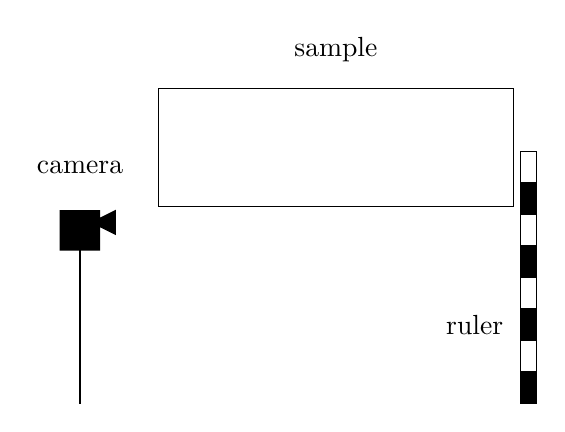
\begin{tikzpicture}
%HORRIBLE camera picture

%displacement
%\draw (1,2.5) parabola bend (3.25,2) (5.5,2.5) node [midway] (down) {this};

%camera
\draw (0,0) -- ++ (0,1.95);
\draw [fill = black]
(-0.25,1.95) rectangle ++ (.5,.5)
(0.25,2.35) -- ++ (0.2,0.1) -- ++ (0,-0.3) -- ++ (-0.2,0.1);

%\draw[ultra thin] (0.25,2.2) -- (5.6,2.4)
%(0.25,2.2) -- (5.6,2);

%sample
\draw
(1,2.5) rectangle ++ (4.5,1.5); 

%ruler
\draw 
(5.6,0) -- (5.6,3.2) -- (5.8,3.2) -- (5.8,0) ;
\foreach \x in {0,0.8, ..., 3.2}
\draw [fill = black]
(5.6,\x) rectangle ++ (0.2,0.4);

%central line
%\draw[ultra thin,dashed] (3.25,4) -- (3.25,0);

%distances
%\draw [{Latex[length=3mm, width=1mm]}-{Latex[length=3mm, width=1mm]}] 
%(0,-1) -- (3.25,-1) node [midway, above] {1,0 m};
%\draw [{Latex[length=3mm, width=1mm]}-{Latex[length=3mm, width=1mm]}] 
%(3.25,-1) -- (5.5,-1) node [midway, above] {0,75 m};
%\draw [{Latex[length=3mm, width=1mm]}-{Latex[length=3mm, width=1mm]}] 
%(0,-2) -- (5.5,-2) node [midway, above] {1,75 m};

%text
\draw (0,3) node {camera}
(3.25,4.5) node {sample}
(5.5,1) node [left] {ruler};

%\draw [{Latex[length=3mm, width=1mm]}-{Latex[length=3mm, width=1mm]}] (3.25,2.5) -- (down);

\end{tikzpicture}